\documentclass{article}
\usepackage{authblk}
\usepackage{blindtext}
\usepackage{listings}
\usepackage{color}
\usepackage{amsmath}
\usepackage{amsthm}
\usepackage{graphicx}
\usepackage{amsmath,amssymb,amsthm}
\usepackage{algorithm}
\usepackage[noend]{algpseudocode}
\newcommand{\limp}{\Rightarrow}
\newcommand{\WP}[2]{\mathit{WP}(#1,#2)}
\newcommand{\SP}[2]{\mathit{SP}(#1,#2)}
\newcommand{\havoc}{\mathit{havoc}}
\newcommand{\guard}{\mathit{guard}}
\definecolor{codegreen}{rgb}{0,0.6,0}
\definecolor{codegray}{rgb}{0.5,0.5,0.5}
\definecolor{codepurple}{rgb}{0.58,0,0.82}
\definecolor{backcolour}{rgb}{0.95,0.95,0.92} 
\lstdefinestyle{mystyle}{
    backgroundcolor=\color{backcolour},   
    commentstyle=\color{codegreen},
    keywordstyle=\color{magenta},
    numberstyle=\tiny\color{codegray},
    stringstyle=\color{codepurple},
    basicstyle=\footnotesize,
    breakatwhitespace=false,         
    breaklines=true,                 
    captionpos=b,                    
    keepspaces=true,                 
    numbers=left,                    
    numbersep=5pt,                  
    showspaces=false,                
    showstringspaces=false,
    showtabs=false,                  
    tabsize=2
}
\newtheorem{mydef}{Definition}
\newtheorem{theorem}{Theorem}
\newtheorem{lemma}{Lemma}
\renewcommand{\algorithmicrequire}{\textbf{Input:}}
\newcommand{\ultimate}{\textsc{Ultimate}\xspace} % Ultimate

\lstset{style=mystyle}
\usepackage[utf8]{inputenc}
\title{Static fault localization for simple bugs \\ \normalsize{(background work)}}
\author{Muhammad Numair Mansur}
\affil{University of Freiburg, Germany}
\date{\vspace{-5ex}}




\begin{document}

\begin{titlepage}
    \begin{center}
        \vspace*{1cm}
        \Large
        \textbf{Static fault localization for simple bugs} \\
        \large
        (background work)
        \vspace{0.5cm}
   
        
        \vspace{5cm}
        \large
        \textbf{Muhammad Numair Mansur}
                
        \vspace{0.5cm}
        
        
        Software Engineering Group\\
        University of Freiburg, Germany
        
    \end{center}
    \vspace{8cm}
    \textbf{Supervision}: Matthias Heizmann, Christian Schilling
\end{titlepage}
% ******************************************** BEGIN DOCUMENT **************************************************************************
\section{Introduction}
This document contains behind the scenes work of our submission in \textit{POPL 2018}, namely "Static fault localization for simple bugs". It contains the previous/failed definitions of relevance that lead us to the final version together with examples that show why the previous definitions did not work. It also shows some examples for which the output of our algorithm is counterintuitive. The document should also serve as  a reference for future work for us. This will also be the submission as my master project report.
\section{Motivation}
Identifying program statements that are the cause for the error is the most time consuming and tedious part of a programmer's debugging routine. This task can be made much simpler if it can be done automatically. The process of automatically finding program statements causing the error is called \textit{fault localization}. A program might be failing because of several reasons which are not necessarily simple (a term elaborated more clearly in the paper) and easy to point out and there might be many ways to fix the bug. We, however, stick to what we call simple bugs. A bug in an error trace is called simple if the modification of a single statement can fix the error. There can be many techniques to help the user narrow down his or her search for the statements  causing the error or \textit{relevant} statements, as we call them in the paper. In this work, we present a new such technique that statically analyzes all the assigning statements in an error trace containting a simple bug and returns those, which when modified can fix this bug.\\
Not only did we want to help the user find simple bugs, we also wanted to formalize the notion of when an assigning statement is relevant in an error trace.
Coming up with a precise formal definition took some iterations. All the previous definitions are also presented in this document along with the reasons of why they were discarded and the examples on which the inconsistency between them and our algorithm became clear.\\
\section{Discarded definitions of relevance}
We developed several definitions of relavance while trying to formally characterize the behaviour of our algorithm. We came across several versions that seemed correct at the time but in reality did not accurately and completely explain our notion of relevance and hence were discarded. We discovered this by coming up with counterexamples where these definitions did not work. This section mentions those discarded definitions and the counterexamples.\\ 
They are in the document primarily for the reason of documenting failed/incorrect versions of our current definition that might be useful in the future as we further develop our understanding of what it means that a statement is relevant in an error trace for a simple bug. \\
For future reference it is easier if we name these definitions. Let us name these approaches with "check" in the end since we declare a statement relevant if they satisfy a localized check. 
\subsection{The restrictive-assume check}
This was our first attempt to formally define a relevant assigning statement. At the time, we had two separate checks for relevance of an assignment statement and a havoc.
\subsubsection{Assignment statement}
An assignment statement was marked relevant, if after replacing that assignment with a havoc, some assume statement in the error trace was becoming restrictive.
\begin{mydef}[Restrictiveness of a statement]
Let \emph{pre} be a state formula, $\pi$ a trace and $i$ a position such that $\pi[i]$ is an assume statement. We call the assume statement $\pi[i]$ \emph{restrictive} iff :
$$sp(pre, \pi[0,i-1]) \not \limp guard(\pi[i])$$
\end{mydef}

\begin{mydef}[Relevance of an assignment statement]
Let $\pi$ be an error trace and $\pi[i]$ be an assignment statement at position $i$ having the form $x:=t$, where $x$ is a variable and $t$ is an expression. Let $\pi'$ be the trace which is obtained by replacing $\pi[i]$ by  $havoc(x)$. Let $pre$ be the error precondition of $\pi$. The assignment statement $\pi[i]$ is \emph{relevant} if there exists some assume statement at position $j > i$ in $\pi'$ such that $\pi'[j]$ is restrictive. 
\end{mydef}

\subsubsection{Havoc statement}
\begin{mydef}[Relevance of a havoc statement]
Let $\pi$ be a feasible error trace and $\pi[i]$ be a $Havoc$ statement at position $i$ having the form $havoc(x)$, where $x$ is a variable. Let $\pi'$ be the trace which is obtained by replacing $\pi[i]$ by an assignment statement $x:=t$, where $x$ is the same variable as in havoc(x) and t is an expression. The havoc statement is \emph{relevant} iff there exists an assignment x:=t such that $\pi'$ is infeasible. That is:
$$sp(true; \pi') \Rightarrow false$$
\end{mydef}


\subsubsection{Examples}
\textbf{Where it works} \\
Below is an example where the above check for relevance correctly marks a statement relevant.
\begin{lstlisting}
foo()
{
	x := 1;
	y := 2;
	z := 3;
	assert(z > 10);
}
\end{lstlisting}
Lines 3 and 4 are not relevant as if we replace them with havoc, no assume in the error trace is becoming restrictive. But if we replace line 5 with $havoc(z)$, then the last (and only) assume statement in the error trace ($assume(z<=10)$) is becoming restrictive. Hence the line with the assignment to $z$ is relevant. \\
\textbf{Where it fails}
\begin{lstlisting}
foo()
{
	x := 1;
	y := 2;
	z := 3;
	havoc z;
	assert(z > 10);
}
\end{lstlisting}
In the above example, every statement is now relevant. If we replace any of the assigning statements with $havoc$, the assume statement in the end is restrictive and not necessarily because of the replacement with havoc but because of the last $havoc(z)$ statement in the program. Hence in this program line 3 and 4 are also relevant.\\
Another example where this approach fails is:
\begin{lstlisting}
procedure main()
{
  y := 42;
  havoc x;
  assume(x >= 0 && y >= 23);
  assert(false);
}
\end{lstlisting}
Here replacing the assignment statement $y:=42$ with $havoc(y)$ has no effect on the restrictiveness of an already restrictive error trace. Hence it should not be relevant here. However, clearly this statement is also responsible for the bug.

\subsection{The blocking-executions check}
We adopted this definition for relevance when we realized that we should take into account the "amount" of restrictiveness of an assume statement instead of just considering if it is getting restrictive or not in a binary fashion.
\begin{mydef}[Execution]\label{mydef:execution_definition}
Let $\pi$ be an error trace of length $n$. An \emph{execution} of $\pi$ is a sequence of states $s_0, s_1, ..., s_n$ such that $(s_i, s_{i+1}) \models T$, where $T$ is the transition formula of $\pi[i]$. \\
Let $\xi$ represent the set of all possible executions of the error trace.
\end{mydef}

\begin{mydef}[Blocking Execution]\label{mydef:blockingexecution_definition}
An execution of a trace $\pi$ of size $n$ is called a \emph{blocking execution} if there exists a sequence of states $s_0, s_1,..., s_j$ where $i<j \leq n$ such that $(s_i, s_{i+1}) \models T[i]$, where $T[i]$ is the transition formula of $\pi[i]$ and there exists an assume statement in the trace $\pi$ at position $j$ such that $s_{j} \not \limp guard(\pi[j])$.
\end{mydef}

\begin{mydef}[Relevance]\label{mydef:relevancy_definition}
Let $\mathcal{B}$ represent the set of all blocking executions of a trace $\pi$. Let there be an assignment statement of the form $x:=t$ at position $i$. Let $\pi'$ represent the trace that we get after replacing $\pi[i]$ with a havoc statement of the form $havoc(x)$ and let $\mathcal{B}'$ represent the set of all blocking executions for $\pi'$.\\
We say that the assignment statement $\pi[i]$ is relevant if the trace after the replacement has strictly more blocking executions than the trace before the replacement in the following sense $$\mathcal{B} \subsetneq \mathcal{B}'$$. 
\end{mydef}
\subsubsection{Examples}
\textbf{Where it works}\\
Consider the failed example from the restrictive-assume check. 
\begin{lstlisting}
procedure foo()
{
  y := 42;
  havoc x;
  assume(x >= 0 && y >= 23);
  assert(false);
}
\end{lstlisting}
The blocking-executions check now correctly says that $y:=42$ is relevant since changing it to havoc gives us more blocking executions than before.\\
\textbf{Where it fails}
\begin{lstlisting}
procedure foo()
{
  y := 10;
  havoc x;
  assume(x > 0);
}
\end{lstlisting}
In this example, the statement $y:=10$ clearly has nothing to do with the error. But changing it to havoc gives us more blocking executions than before and according to the blocking-executions check, it is wrongly marked as relevant, too. 

\newpage
\section{Algorithmic modification}
We also noticed that we need a slight modification in the algorithm if we want to make it completley consistent with our notion of relevance. Consider the following example:
\begin{lstlisting}
procedure foo()
{
	x := 5;
	y := 7;
	assume(x != 5 && y != 7)
}
\end{lstlisting}
with an error trace:
\begin{lstlisting}
	x := 5		y := 7		assume (x == 5 || y == 7) 
\end{lstlisting}
According to our final definition of relevance, $y:=7$ should not be relevant as no value $v$ exists such that if we replace $y:=7$ with $y:=v$, the rest of the trace (starting in the state $x=5$) has a blocking execution. 

But our previous algorithm marked the statement as relevant because $P$ was computed as $pre(true, \pi[i,n])$, where $\pi[i]$ is the assignment statement under consideration. Hence $P$ would be $true$ and $Q$ would be $x=5 \vee y=7$. Obviously $P \not \subseteq wp(Q; havoc(y))$, where $wp(Q, havoc(y))$ is $x=5$. Therefore, the assignment is marked relevant. \\
We fixed this error in the algorithm by computing $P$ not as $pre(true, \pi[i,n])$ but as the intersection of $pre(true, \pi[i,n])$ and $sp(true, \pi[0,i-1])$.




\section{Final version of Relevance}
\subsection{Introduction}
An assigning statement ($x := t$ or $havoc(x)$) is responsible in an error trace if the assigned value matters for the reachabilty of the error. If the error state is reachable for any possible value of the variable $x$, then we say that the assignment to $x$ at this location in the error trace is not relevant. Also, in the final version, we have one definition for both the assignment statement and havoc. 
\subsection{Formal definition}
\begin{mydef}[Execution]\label{mydef:execution}
Let $\pi$ be an error trace of length $n$. An execution of $\pi$ is a sequence of states $s_0, s_1,...,s_n$ such that $(s_i, s_{i+1}) \vDash T$, where $T$ is the transition formula of $\pi[i]$.
\end{mydef}
\begin{mydef}[Blocking Execution]\label{mydef:blocked_execution}
An execution of a trace $\pi$ of size $n$ is called a \emph{blocking execution} if there exists a sequence of states $s_0,s_1,...,s_j$ where $i<j \leq n$ such that $(s_i, s_{i+1}) \vDash T$ where $T$ is the transition formula of $\pi[i]$ and there exists an assume statement in the trace $\pi$ at position $j$ such that $s_j \not \limp guard(\pi[j])$
\end{mydef}

\begin{mydef}[Relevance of an assigning statement]\label{mydef:responsible}
Let $\pi = \langle st_1,....,st_n \rangle$ be an error trace of length $n$ where $st_i$ is an assigning statement at position $i$ that assigns a new value to some variable $x$. The statement $st_i$ is relevant if there exists an execution $s_1,...,s_{n+1}$ of $\pi$ and some value $v$ such that every execution of the trace $\langle x:=v; \pi[i+1,n] \rangle$ starting in $s_i$ is blocking.
\end{mydef}

\begin{algorithm}
\caption{Relevance of an assigning statement}\label{relevance}
\begin{algorithmic}[1]
\Procedure{Relevance}{}
\State $trace \gets \text{Error trace } \pi \text{ of length } \textit{n}$
\State $relevantStatements \gets \text{[ ]}$
\For{$i = n$ to $1$}
\State $Q \gets \neg wp(false;trace[i+1,n])$
\State $P \gets wp(Q; trace[i]) \cap sp(true; trace[0;i-1])$
\If{$trace[i]$ is an assigning statement and $P \not \subseteq wp(Q; havoc(x))$ }
\State $relevantStatements.append(trace[i])$
\EndIf
\EndFor
\Return $relevantStatements$
\EndProcedure
\end{algorithmic}
\end{algorithm}
% ******************************************** NEW Page****************************************************************
\begin{theorem}[Equivalence of relevance]\label{mydef:relevancytheorem}
Let $\pi = \langle st_1,...,st_i,...,st_n \rangle$ be an error trace of length $n$ and $\pi[i]$ be an assigning statement at position $i$ that assigns a new value to some variable $x$. Let $P = \neg WP(false; \pi[i,n]) \cap SP(true; \pi[0,i-1])$ be a set of bi-reachable states at position $i$ and $Q =  \neg WP(false; \pi[i+1,n])$ be the co-reachable states at position $i+1$. The statement $\pi[i]$ is relevant iff:
 $$P \not \subseteq WP(Q,havoc(x))$$
\end{theorem}

\begin{proof}
Let $\mathcal{D}$ be the domain of the variable $x$. \\
"$\Rightarrow$"\\
If $\pi[i]$ is relevant, then we have to show that\\
$$P \not \subseteq WP(Q;havoc(x))$$
Obviously all the transitions from the states in $WP(Q;havoc(x))$ end up in $Q$. Relevance of $\pi[i]$ implies that there is a state $s$ in $P$ such that there is a transition from $s$ to $\neg Q$. That would mean:
$$P \not \subseteq WP(Q;havoc(x))$$
"$\Leftarrow$"\\
$\pi[i]$ is relevant, if:
$$P \not \subseteq WP(Q;havoc(x))$$
We know that $WP(Q;havoc(x))$ is the set of states from which all transitions end up in $Q$. The above non-implication shows the existence of a state $s$ in $P$ such that $s \not \in WP(Q; havoc(x))$  from which there is a transition to $\neg Q$. This shows the existence of a value $v \in \mathcal{D}$ that we can assign to $x$ such that if we replace $\pi[i]$ with $x:=v$, then every execution starting from $s$ is becoming blocking. Also, from our assumption, it is clear that there exists an execution till $s$, since $P$ is not empty.
\end{proof}

\subsection{Examples}
Consider the failed examples from previous definitions and let us analyze them again under our new definition.
\begin{lstlisting}
foo()
{
	x := 1;
	y := 2;
	z := 3;
	havoc z;
	assert(z > 10);
}
\end{lstlisting}
In the example above which contains only one error trace and where the restrictive-assume check fails, only the havoc statement at line 6 is now relevant according to our new definition. \\
\\
Consider the example where the blocking-executions check failed:
\begin{lstlisting}
foo()
{
  y := 10;
  havoc x;
  assert(x > 0);
}
\end{lstlisting}
Only $havoc(x)$ is now relevant since there is no assignment to $y$ in line 3 that can make an existing execution of the error trace blocking.


\section{Possibly counter-intuitive cases}
This section mentions three examples with  counter-intuitive results when analyzed by our algorithm. All the examples can be found in \ultimate repository's examples folder for Error localization. For future reference, let us name these examples as follows:
\subsection{Two-havoc case}
Consider the following program:
\begin{lstlisting}
procedure foo()
{
	havoc x;
	havoc y;
	assert(x>0 && y>0)
}
\end{lstlisting}
Our algorithm only consider the second havoc as relevant. This seem rather surprising at first sight but consider an execution of the error trace where $x$ is assigned the value 1\\
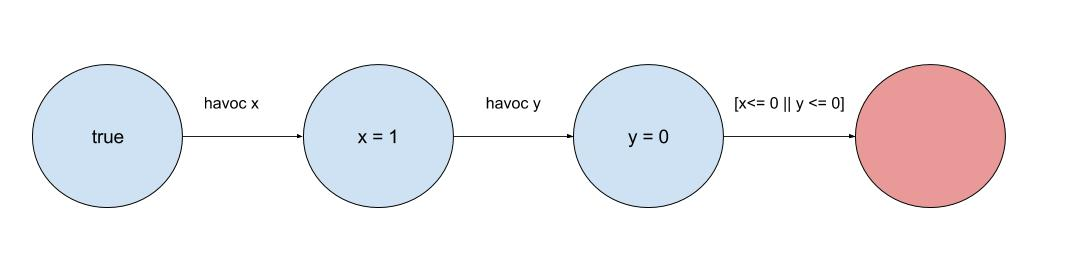
\includegraphics[width=\linewidth]{2havocs1.jpg}\\

\subsection{Relevant-havoc case}
Consider the following program:
\begin{lstlisting}
procedure foo(a,b)
{
    havoc x;
    if(x > 10){
      x := x+1;
    }
    else {
      x := x-1;
    }
    assert a > b;
}
\end{lstlisting}
Our algorithm considers havoc x relevant even tough fixing this statement will not fix the error.

\subsection{Two-assignment case}
Consider the following example:
\begin{lstlisting}
procedure foo()
{
    x := 10;
    y := 10;
    assert x < 10 && y < 10;
}
\end{lstlisting}
In this case none of the assignment statements are relevant since the assume statement in the end would have a disjunction and none of the assignment statements can make the assume blocking. 
\section{Known problems}
Currently, our implementation in \ultimate fails to give expected results when array modification is involved in the program. This is due to the fact that we can havoc the whole array at the moment and not one element. Due to this problem, if any assignment to an array element is relevant according to our algorithm, all the assignments that modify any element of the same array will be returned as relevant as well. The following example will make this problem more clear:
\begin{lstlisting}
foo()
{ 
  havoc j;
  i := j + 1;
  a[i] := 5;
  a[j] := 7;
  assert(a[i] == 8);
}
\end{lstlisting}
The implementation marks both the assignment statements modifying the array elements as relevant.

\section{Comparison with other approaches}
\subsection{Error Invariants}
One weakness of the error invariants approach \cite{errorinvariants} is it's inability to deal with havoc statements. The other weakness is related to the fact that generating error invariants require an unsatisfiable trace formula. This leads to a limitation in the case when there is an assert false at the end of that unsatisfiable trace formula. In this case, all the interpolants can be chosen as true and none of the statements would be considered relevant. We call this the \textit{assert-false problem}. Following is a very simple example where this problem becomes easy to see:
\begin{lstlisting}
foo()
{ 
	x := 1;
	if(x < 10)
	{
		assert false;	
	}	
}
\end{lstlisting}
All the interpolants can be chosen as true and $x:=1$ would not be considered relevant in this case. Following example is a characterization of the assert-false problem.
\begin{lstlisting}
foo()
{ 
	p1 := -1;
	i := 1; //  Bug:i should be 0
	while(i < 10){
		if(i==0){
			p1 := 0;		
		}
		assert( p1 != -1):
		i++;	
	}
}
\end{lstlisting}
In this example, only line 3 would be considered relevant according to the error invariants approach. Where as the bug is that the user actually forgot to initialize $i$ with 0. Our algorithm was however able to catch this problem. This is also the example we used in the \textit{POPL} submission but with an extra variable p2.

\subsection{Flow Sensitive Fault localization} 
In the paper flow sensitive fault localization\cite{faultlocalization}, the authors try to take into account the control flow of the program and propose a flow sensitive error localization technique which, they hope, not only explain the cause of the error but also explain why the statements leading to the error were executed. They do this by modifying the so called \textit{error trace formula} to something which they call a \textit{flow sensitive error trace formula}. An error trace formula is just a conjunction of the trace formula of the error trace together with the error precondition and the correctness assertion. Information about the relevant statements can be obtained from the proof of unsatisfiability of the error trace formula.

The flow sensitive error trace formula is a modification of the error trace formula, such that it now keeps track of dependencies between statements and the branching conditions that are relevant for the reachability of these statements in the control flow graph of the program. \\
The main focus of the authors here is on finding the relevant assume statements and the statements that cause the guard of the relevant assume statements to hold. We on the other hand only focus on the statements that cause the state of the program to change and do not analyze assume statements directly. However, we are still able to find the assignment statements that cause the guard of the relevant assume statements to hold. Let us look at an example where our algorithm can already find the statements which the authors can find only after modifying there formula. 
\begin{lstlisting}
foo()
{
	x := 1;
	y := input - 42;
	if (y < 0) {
		x := 0;	
	}
	assert(x != 0);
}
\end{lstlisting}
Both the flow sensitive approach and our algorithm say that the assignment statements $y := input - 42$ and $x := 0$ are relevant for the error.
\section{Future work}
\subsection{Call/Return statements}
We yet have to see the behaviour of our algorithm during procedure calls and define when a call and return statement should be relevant in an error trace. This would require some deeper study and would therefore be considered in future work.
\subsection{Security Analysis}
An interesting problem that we might be able to solve is to distinguish security bugs from non-security bugs. According to our initial understanding, a bug is a security bug iff an input (network/user) statement can cause the program execution to reach the error state. \\
Following are the possible criterion for a bug to be called a security bug.
\begin{enumerate}
  \item There  is some reachable location where a program reads an input.
  \item There is some input value, such that continuing from this location we definitely reach the error.
  \item There is some input that continuing from this location we do not reach the error.
\end{enumerate}
From condition 2 and 3, we can conclude that the input is somehow relevant for the error. This is of course just our initial understanding on this topic, which may not be accurate and further work is needed to formally define a security bug which would involve analyzing in detail the examples that contain security bugs.
\newpage

\begin{thebibliography}{9}
\bibitem{errorinvariants} 
E.Ermis, M. Schaf, and T. Wies. Error Invariants. In FM’12, pages 338–353. Springer, 2012.
\bibitem{inconsistentcode}
M. Schaf, D. Schawrtz, T. Wies. Explaining Inconsistent Code. In Joint meeting of the European Software Engineering conference and the Symposium on the Foundations of Software Engineering, ESEC/FSE’13, pages: 521 - 531, Saint Petersburg, Russian Federation. August 18-26,2013 
\bibitem{faultlocalization} 
J. Christ, E. Ermis, M. Schaf, and T. Wies. Flow-sensitive fault localization. In VMCAI, volume 7737, pages 189–208, Berlin, Heidelberg, 2013. Springer 
\end{thebibliography}
\end{document}